\documentclass{article}
\usepackage{graphicx}
\usepackage[utf8]{inputenc}
\usepackage[T1]{fontenc}
\usepackage{lmodern}
\usepackage{float}
\usepackage{caption}
\usepackage{subcaption}
\usepackage[paperwidth=4.1in, paperheight=5.8in, margin=0.25in]{geometry}
\renewcommand*\familydefault{\sfdefault}
\pagenumbering{gobble}

\usepackage{pgfmorepages}

\pgfpagesdeclarelayout{8 on 2, book format}
{%
  \edef\pgfpageoptionheight{\the\paperheight}
  \edef\pgfpageoptionwidth{\the\paperwidth}
  \def\pgfpageoptionborder{0pt}
  \def\pgfpageoptionfirstshipout{1}
}%
{%
  \pgfpagesphysicalpageoptions
  {%
    logical pages=8,%
    physical pages=2,%
    physical height=\pgfpageoptionheight,%
    physical width=\pgfpageoptionwidth,%
    current logical shipout=\pgfpageoptionfirstshipout%
  }
  \pgfpagesphysicalpage{1}{}
    \pgfpageslogicalpageoptions{4}
    {%
      border shrink=\pgfpageoptionborder,%
      resized width=.5\pgfphysicalwidth,%
      resized height=.5\pgfphysicalheight,%
      center=\pgfpoint{.25\pgfphysicalwidth}{.75\pgfphysicalheight}%
    }%
    \pgfpageslogicalpageoptions{2}
    {%
      border shrink=\pgfpageoptionborder,%
      resized width=.5\pgfphysicalwidth,%
      resized height=.5\pgfphysicalheight,%
      center=\pgfpoint{.75\pgfphysicalwidth}{.75\pgfphysicalheight}%
    }%
    \pgfpageslogicalpageoptions{8}
    {%
      border shrink=\pgfpageoptionborder,%
      resized width=.5\pgfphysicalwidth,%
      resized height=.5\pgfphysicalheight,%
      center=\pgfpoint{.25\pgfphysicalwidth}{.25\pgfphysicalheight},%
    }%
    \pgfpageslogicalpageoptions{6}
    {%
      border shrink=\pgfpageoptionborder,%
      resized width=.5\pgfphysicalwidth,%
      resized height=.5\pgfphysicalheight,%
      center=\pgfpoint{.75\pgfphysicalwidth}{.25\pgfphysicalheight},%
    }%
  \pgfpagesphysicalpage{2}{}
    \pgfpageslogicalpageoptions{1}
    {%
      border shrink=\pgfpageoptionborder,%
      resized width=.5\pgfphysicalwidth,%
      resized height=.5\pgfphysicalheight,%
      center=\pgfpoint{.25\pgfphysicalwidth}{.75\pgfphysicalheight}%
    }%
    \pgfpageslogicalpageoptions{3}
    {%
      border shrink=\pgfpageoptionborder,%
      resized width=.5\pgfphysicalwidth,%
      resized height=.5\pgfphysicalheight,%
      center=\pgfpoint{.75\pgfphysicalwidth}{.75\pgfphysicalheight}%
    }%
    \pgfpageslogicalpageoptions{5}
    {%
      border shrink=\pgfpageoptionborder,%
      resized width=.5\pgfphysicalwidth,%
      resized height=.5\pgfphysicalheight,%
      center=\pgfpoint{.25\pgfphysicalwidth}{.25\pgfphysicalheight},%
    }%
    \pgfpageslogicalpageoptions{7}
    {%
      border shrink=\pgfpageoptionborder,%
      resized width=.5\pgfphysicalwidth,%
      resized height=.5\pgfphysicalheight,%
      center=\pgfpoint{.75\pgfphysicalwidth}{.25\pgfphysicalheight},%
    }%
}


\pgfpagesuselayout{8 on 2, book format}[a4paper]
\begin{document}
    
        \par\noindent\rule{\textwidth}{0.4pt}
    \begin{figure}[H]
        \centering
        \begin{minipage}{0.25\textwidth}
            \centering
            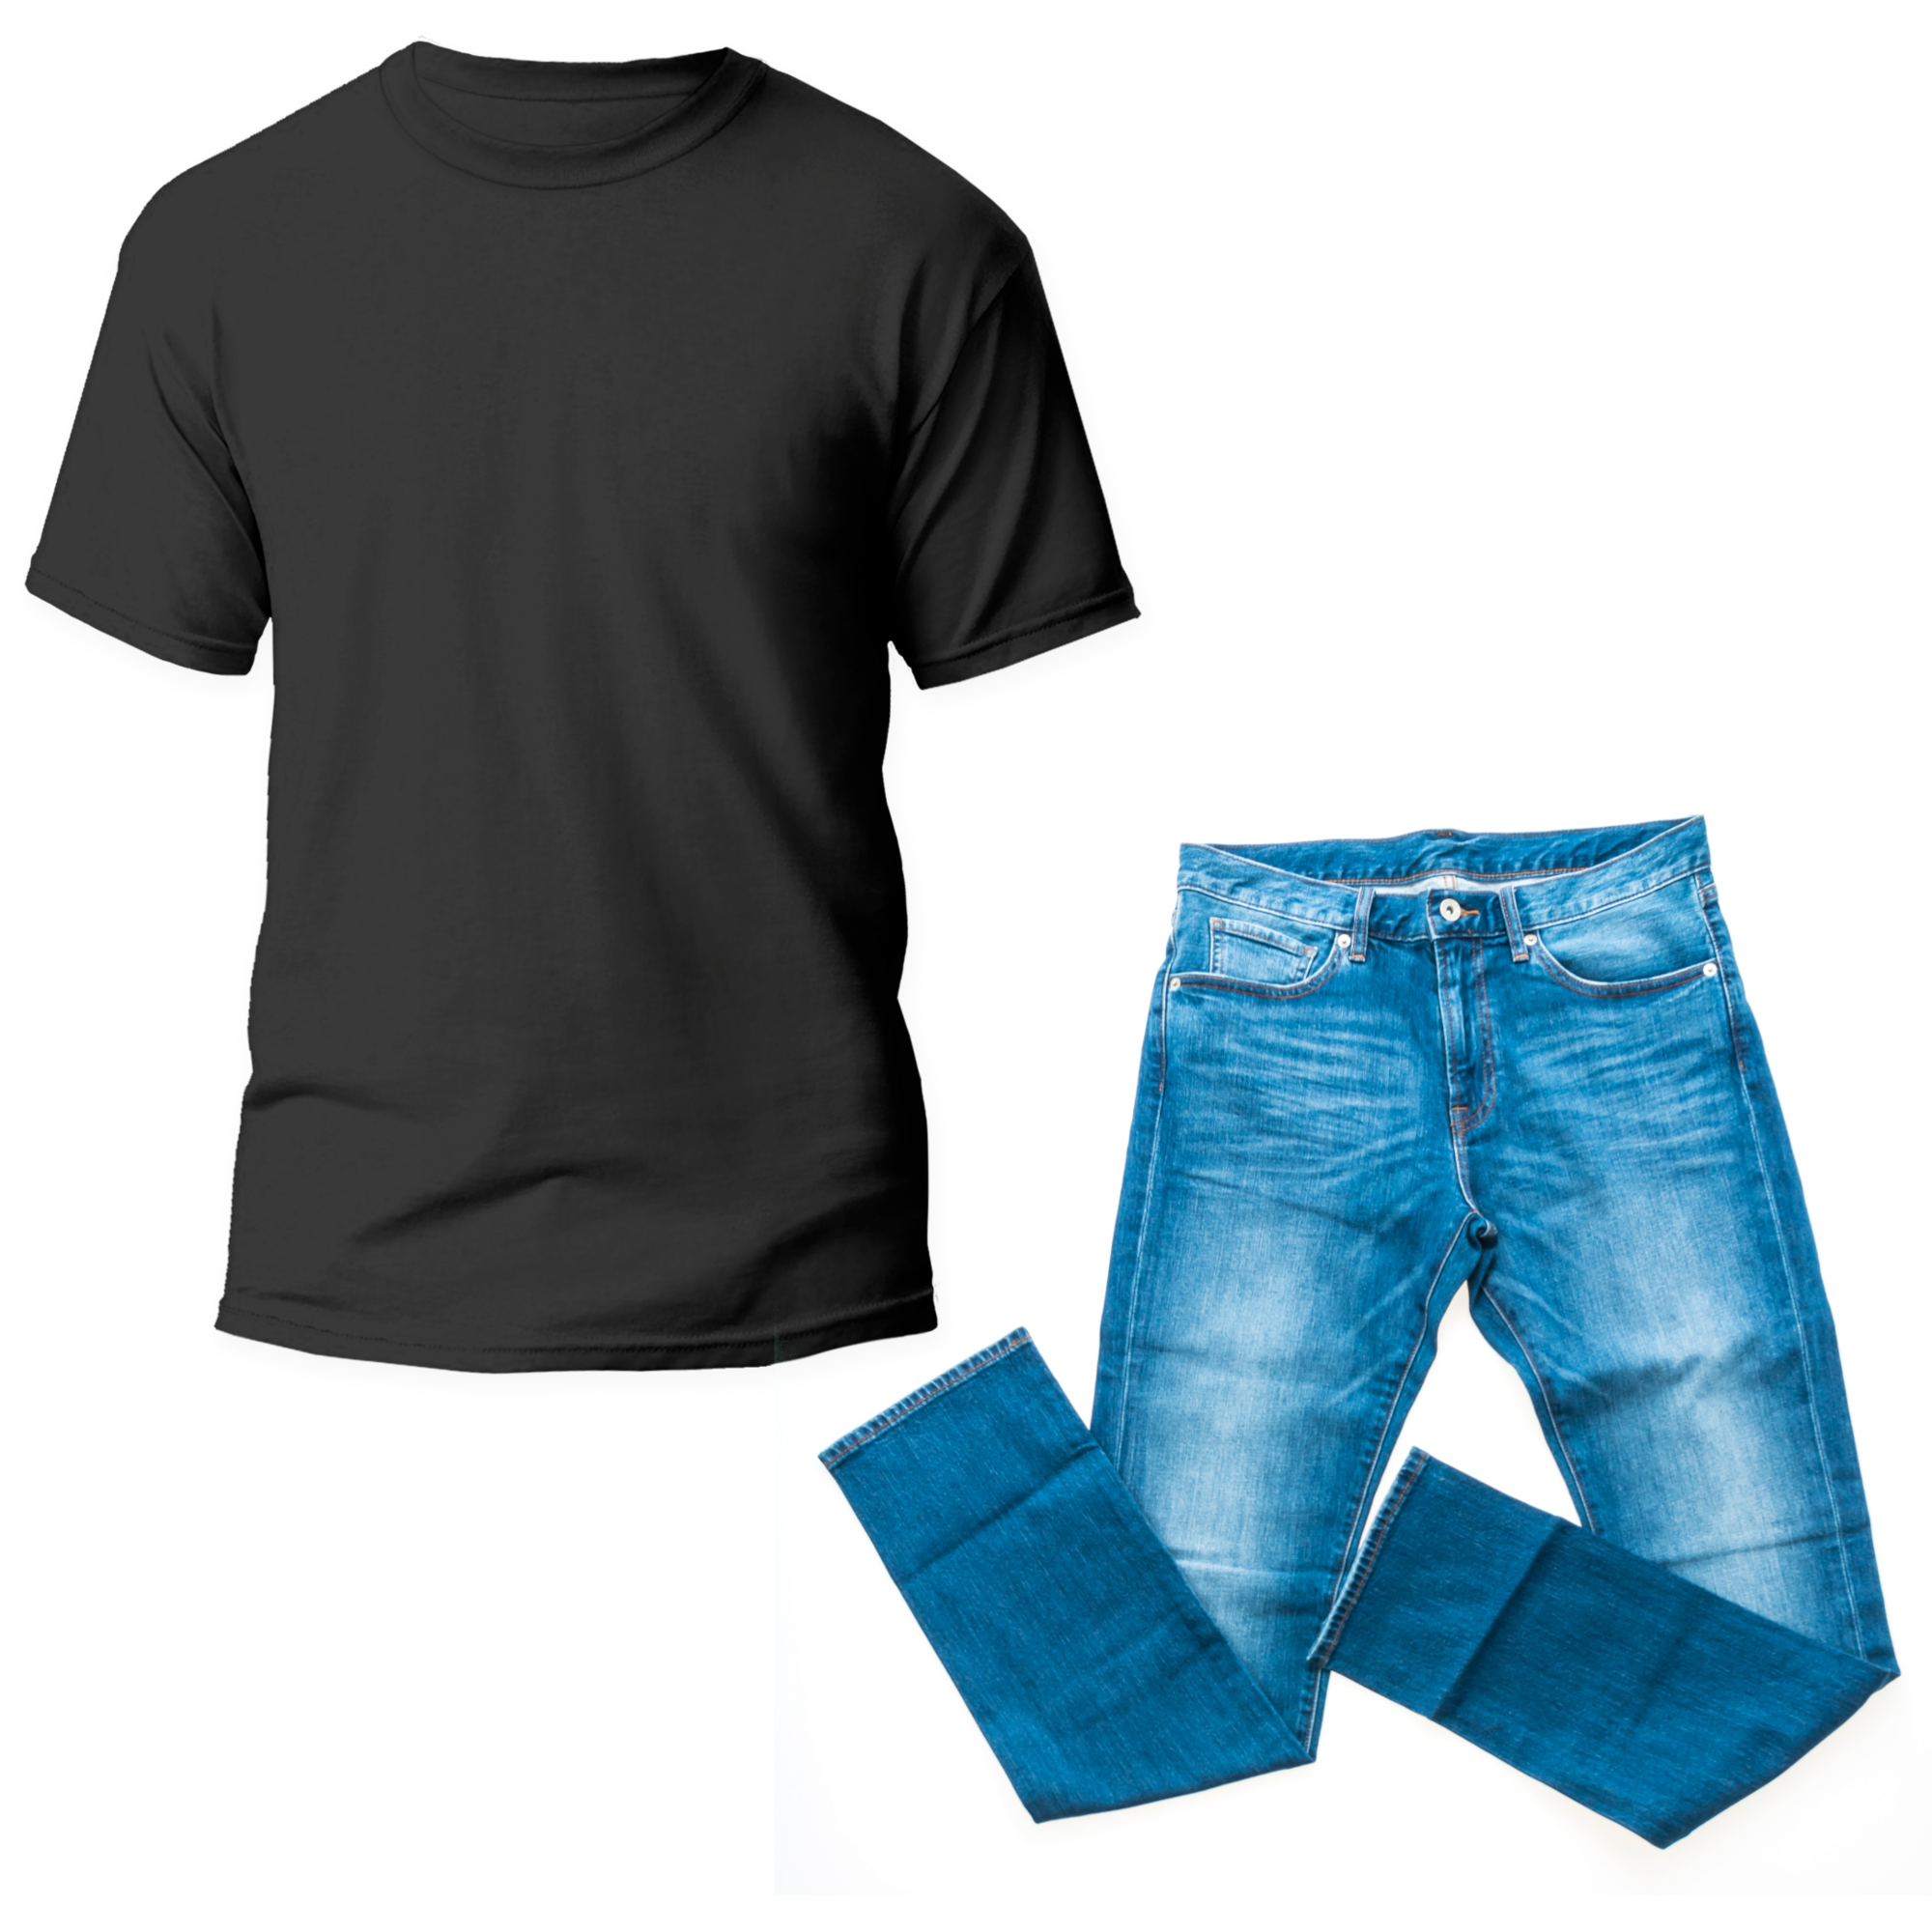
\includegraphics[width=\textwidth]{../SurvivalItemImages/shirt_trousers}
        \end{minipage}\hfill
        \begin{minipage}{0.7\textwidth}
            \centering
            \Large Extra shirt and pants for each survivor
        \end{minipage}
    \end{figure}
    \vspace{-0.8em}
    \noindent\rule{\textwidth}{0.4pt}
            
    \begin{figure}[H]
        \centering
        \begin{minipage}{0.25\textwidth}
            \centering
            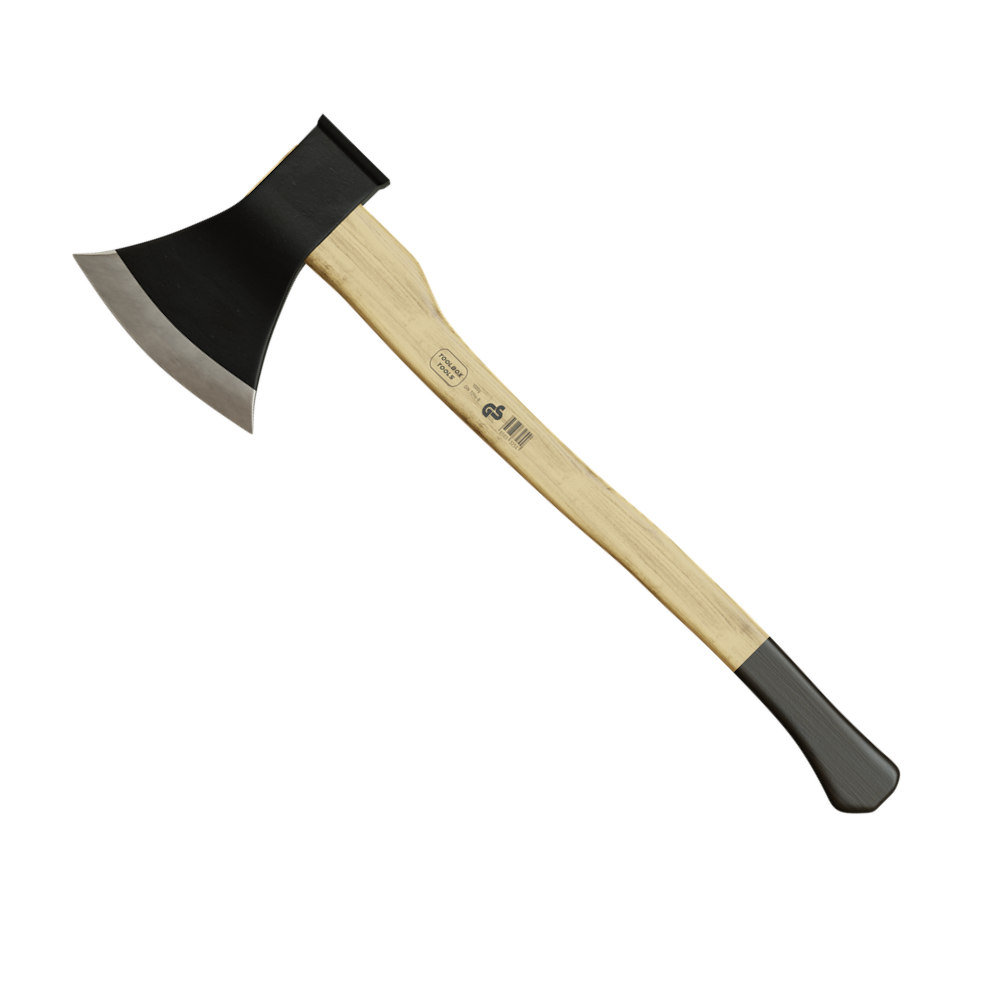
\includegraphics[width=\textwidth]{../SurvivalItemImages/axe}
        \end{minipage}\hfill
        \begin{minipage}{0.7\textwidth}
            \centering
            \Large A little axe
        \end{minipage}
    \end{figure}
    \vspace{-0.8em}
    \noindent\rule{\textwidth}{0.4pt}
            
    \begin{figure}[H]
        \centering
        \begin{minipage}{0.25\textwidth}
            \centering
            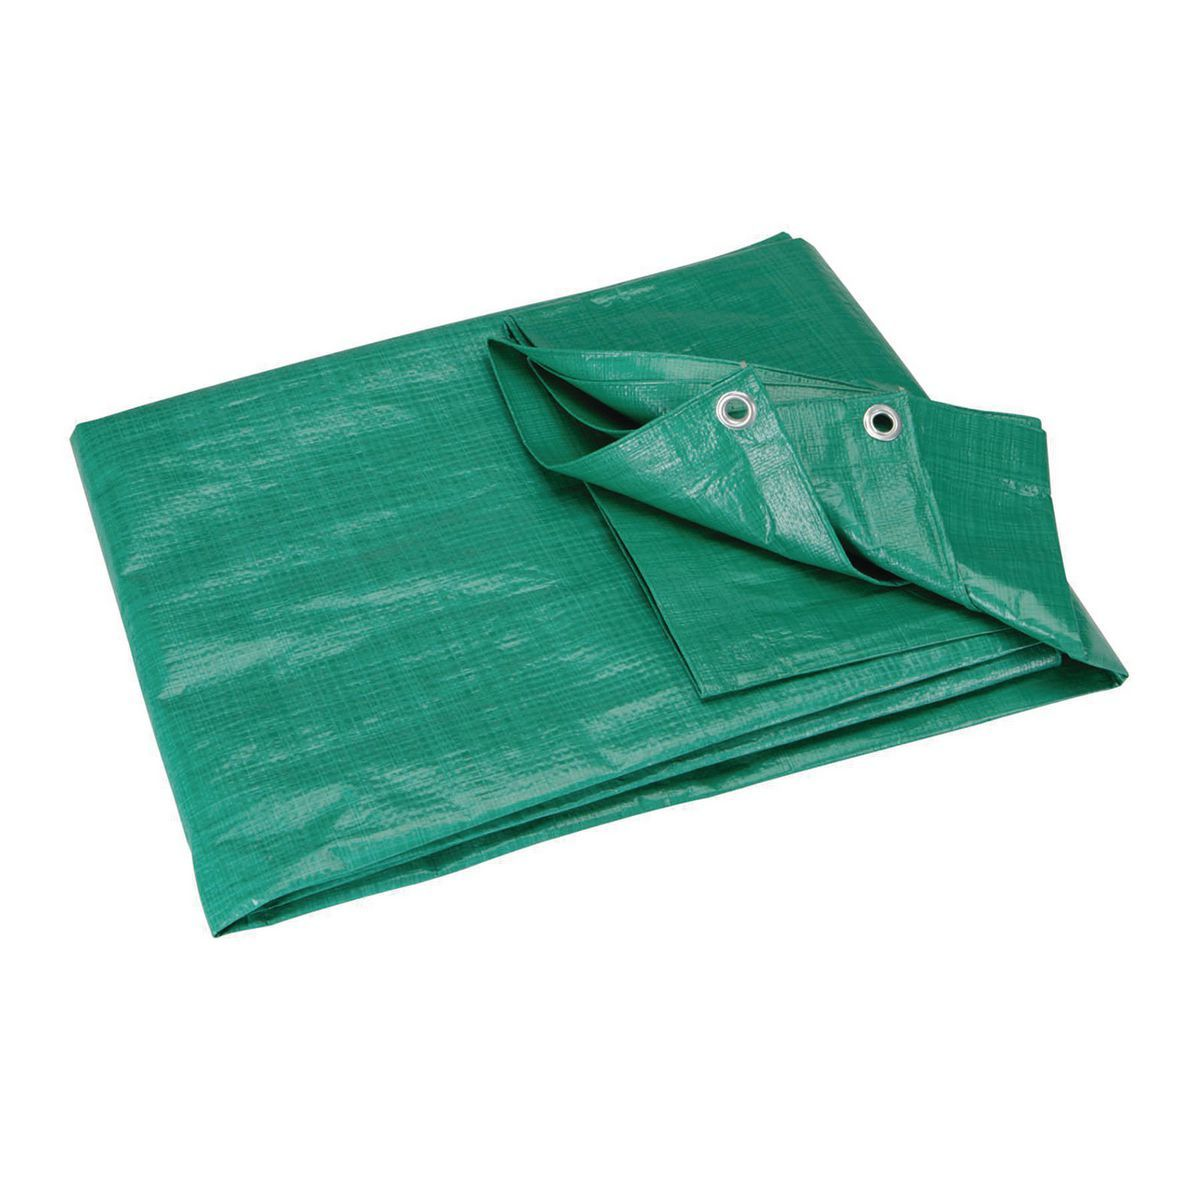
\includegraphics[width=\textwidth]{../SurvivalItemImages/tarp}
        \end{minipage}\hfill
        \begin{minipage}{0.7\textwidth}
            \centering
            \Large A strong sheet (6 m x 6 m)
        \end{minipage}
    \end{figure}
    \vspace{-0.8em}
    \noindent\rule{\textwidth}{0.4pt}
            
    \begin{figure}[H]
        \centering
        \begin{minipage}{0.25\textwidth}
            \centering
            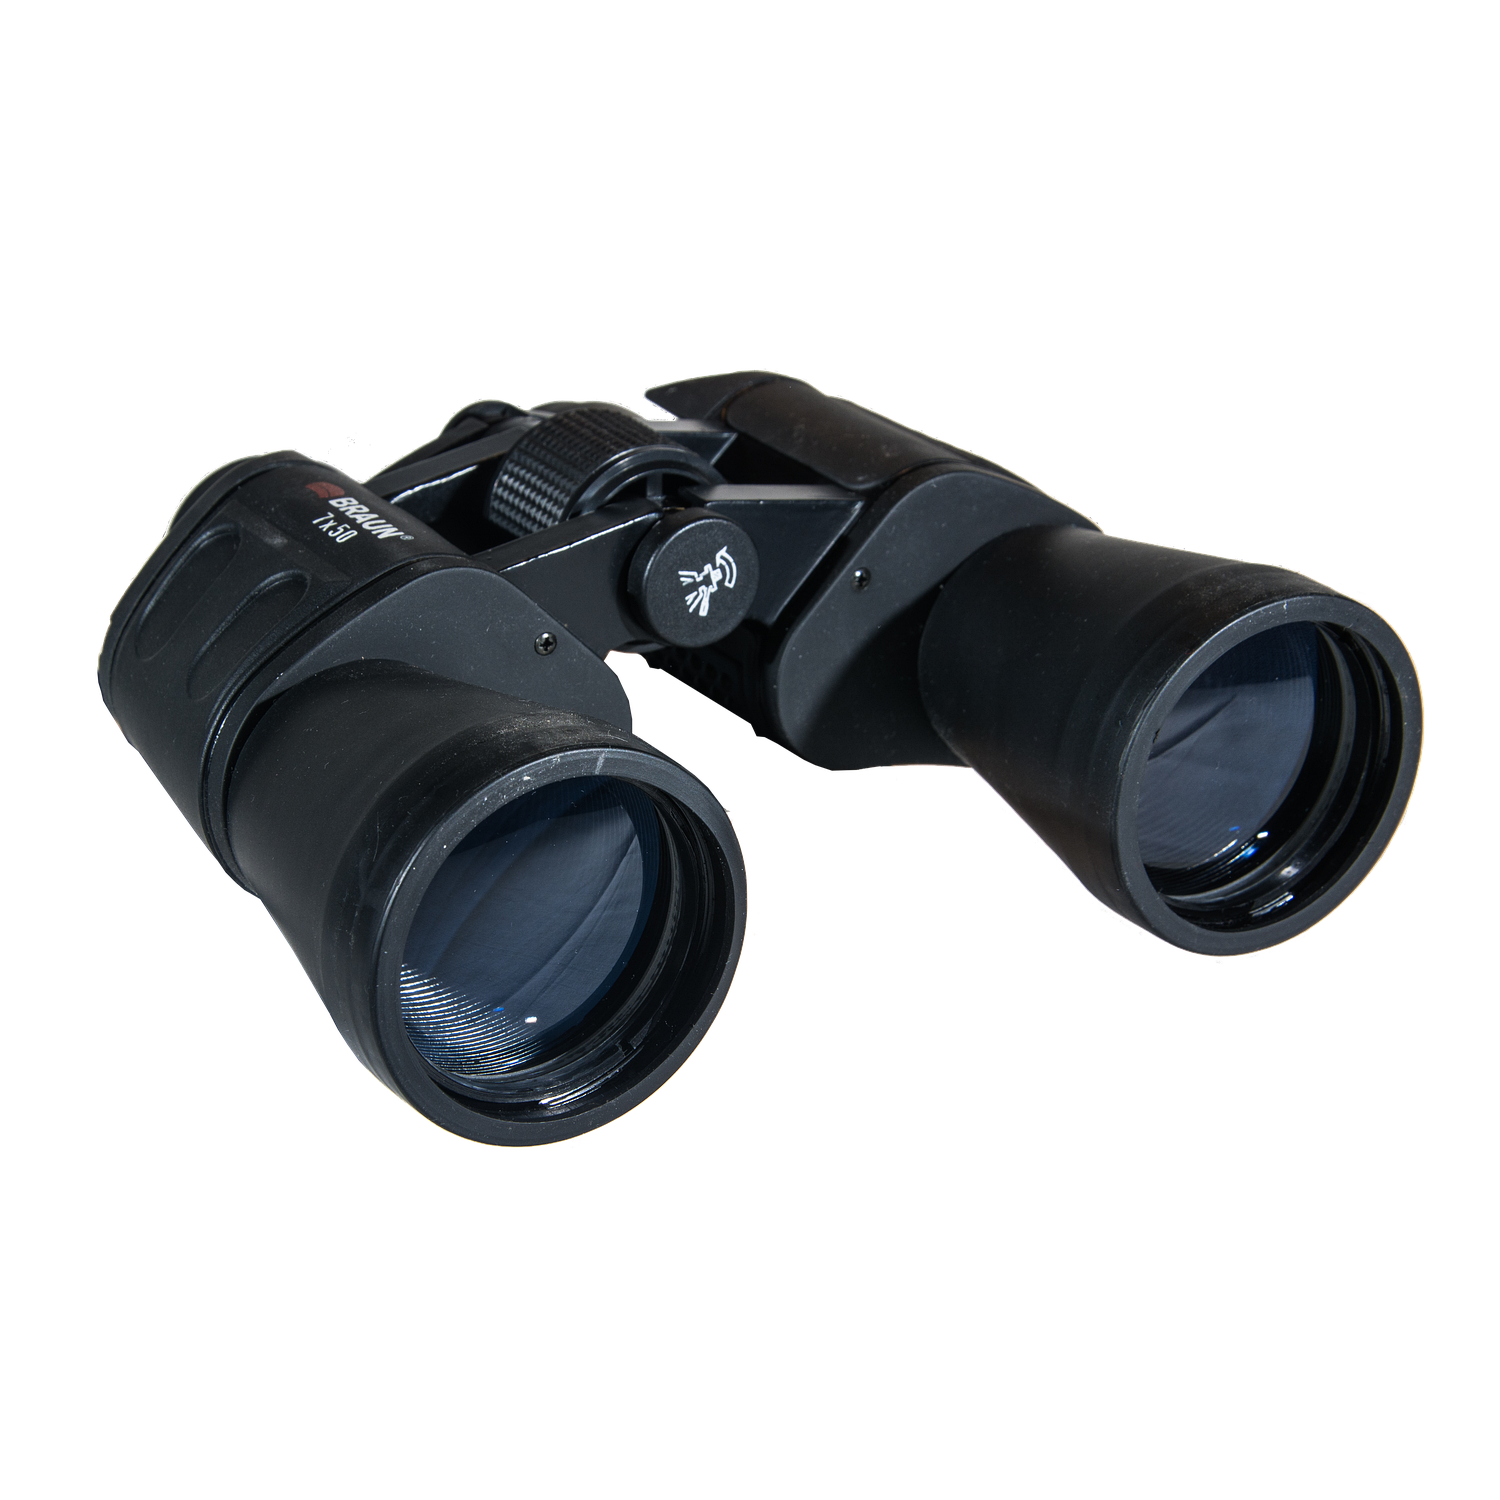
\includegraphics[width=\textwidth]{../SurvivalItemImages/binoculars}
        \end{minipage}\hfill
        \begin{minipage}{0.7\textwidth}
            \centering
            \Large Binoculars
        \end{minipage}
    \end{figure}
    \vspace{-0.8em}
    \noindent\rule{\textwidth}{0.4pt}
            
    \clearpage
    \section*{Scenario: \textmd{Winter} \hfill Participant \textmd{0}}
    \Large You have just crash-landed in the North of Canada. The small plane in which you were travelling has been completely destroyed except for the frame. The pilot and co-pilot have been killed, but no one else is seriously injured.
You are in a wilderness area, snow-covered and made up of thick woods broken by many lakes and rivers. The pilot announced shortly before the crash that you were eighty miles northwest of a small town that is the nearest known habitation. It is mid-January. The last weather report indicated that the temperature would reach minus twenty-five degrees in the daytime and minus forty at night. You are dressed in winter clothing appropriate for city wear – suits, pantsuits, street shoes, and overcoats. While escaping from the plane, your group salvaged a few items.
\clearpage
        \par\noindent\rule{\textwidth}{0.4pt}
    \begin{figure}[H]
        \centering
        \begin{minipage}{0.25\textwidth}
            \centering
            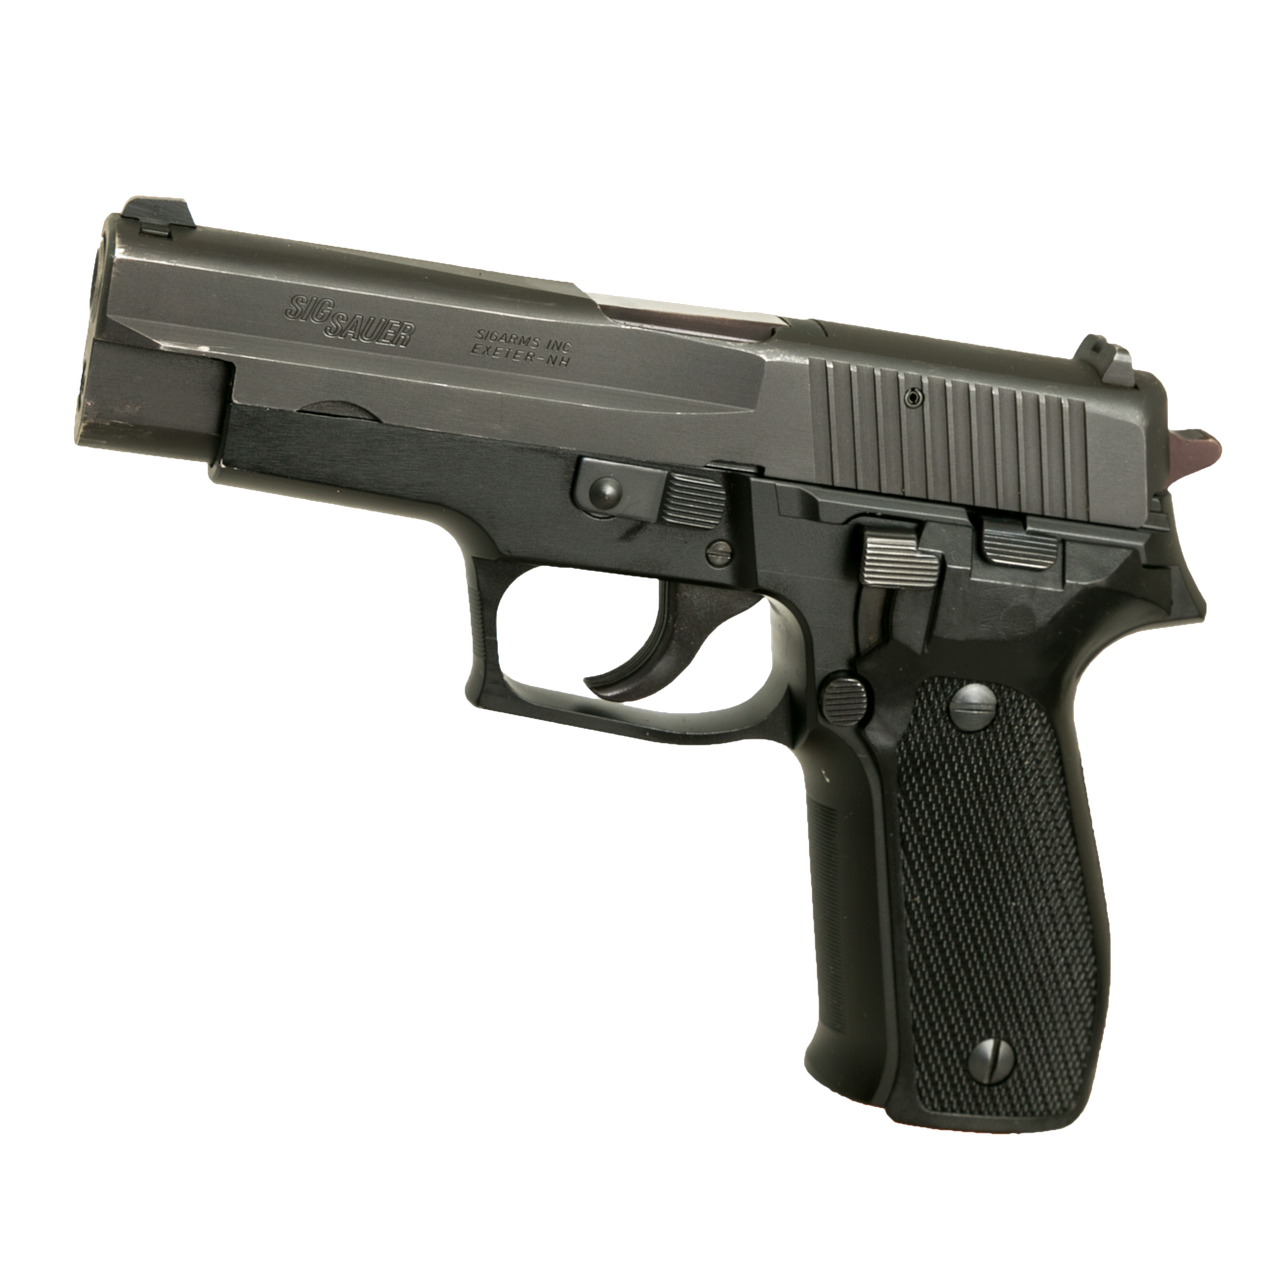
\includegraphics[width=\textwidth]{../SurvivalItemImages/pistol}
        \end{minipage}\hfill
        \begin{minipage}{0.7\textwidth}
            \centering
            \Large Loaded .45-calibre pistol
        \end{minipage}
    \end{figure}
    \vspace{-0.8em}
    \noindent\rule{\textwidth}{0.4pt}
            
    \begin{figure}[H]
        \centering
        \begin{minipage}{0.25\textwidth}
            \centering
            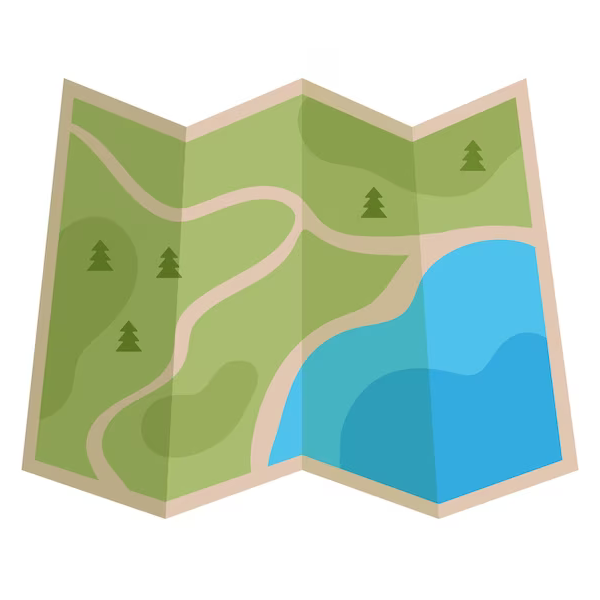
\includegraphics[width=\textwidth]{../SurvivalItemImages/map}
        \end{minipage}\hfill
        \begin{minipage}{0.7\textwidth}
            \centering
            \Large Sectional air map made of plastic
        \end{minipage}
    \end{figure}
    \vspace{-0.8em}
    \noindent\rule{\textwidth}{0.4pt}
            
    \begin{figure}[H]
        \centering
        \begin{minipage}{0.25\textwidth}
            \centering
            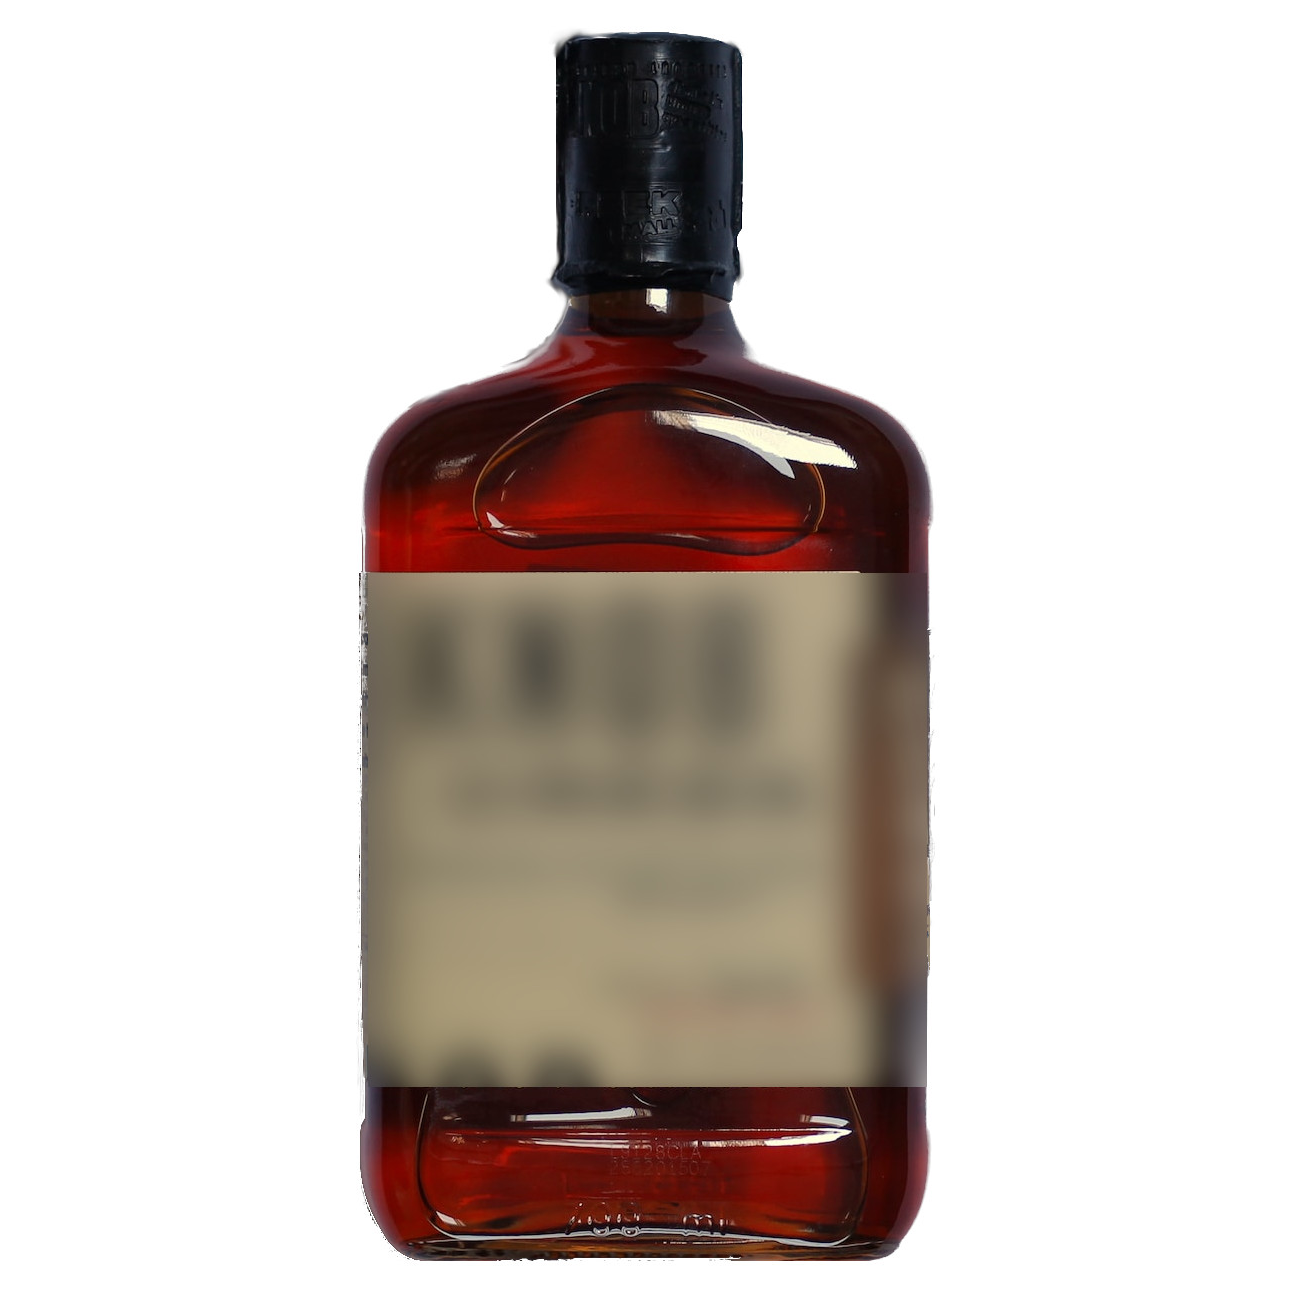
\includegraphics[width=\textwidth]{../SurvivalItemImages/whiskey}
        \end{minipage}\hfill
        \begin{minipage}{0.7\textwidth}
            \centering
            \Large Quart of 85-proof whiskey
        \end{minipage}
    \end{figure}
    \vspace{-0.8em}
    \noindent\rule{\textwidth}{0.4pt}
            
    \begin{figure}[H]
        \centering
        \begin{minipage}{0.25\textwidth}
            \centering
            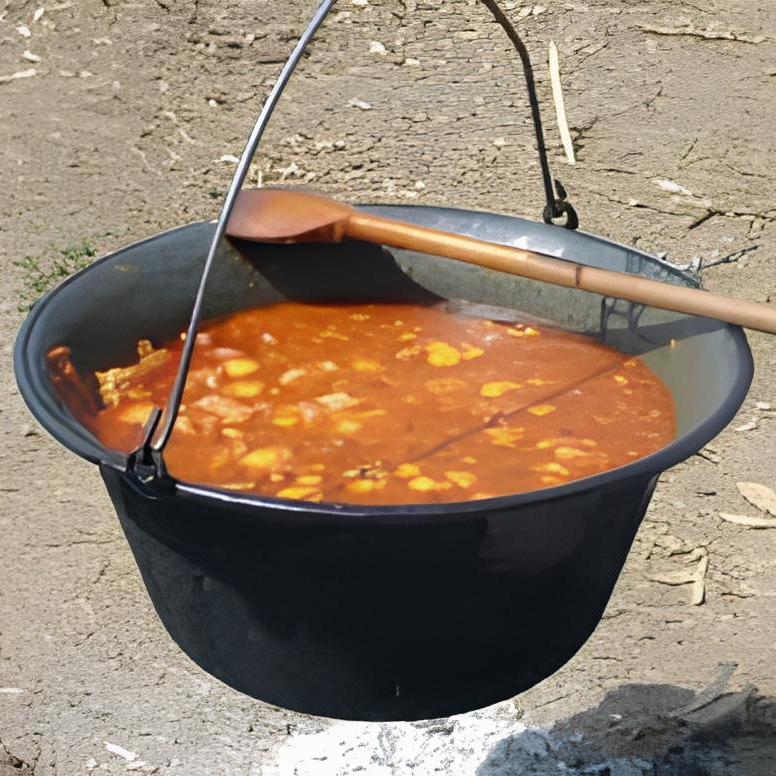
\includegraphics[width=\textwidth]{../SurvivalItemImages/pot}
        \end{minipage}\hfill
        \begin{minipage}{0.7\textwidth}
            \centering
            \Large A camping kettle with mounting
        \end{minipage}
    \end{figure}
    \vspace{-0.8em}
    \noindent\rule{\textwidth}{0.4pt}
            
    \clearpage
    \section*{Scenario: \textmd{Winter} \hfill Participant \textmd{1}}
    \Large You have just crash-landed in the North of Canada. The small plane in which you were travelling has been completely destroyed except for the frame. The pilot and co-pilot have been killed, but no one else is seriously injured.
You are in a wilderness area, snow-covered and made up of thick woods broken by many lakes and rivers. The pilot announced shortly before the crash that you were eighty miles northwest of a small town that is the nearest known habitation. It is mid-January. The last weather report indicated that the temperature would reach minus twenty-five degrees in the daytime and minus forty at night. You are dressed in winter clothing appropriate for city wear – suits, pantsuits, street shoes, and overcoats. While escaping from the plane, your group salvaged a few items.
\clearpage
        \par\noindent\rule{\textwidth}{0.4pt}
    \begin{figure}[H]
        \centering
        \begin{minipage}{0.25\textwidth}
            \centering
            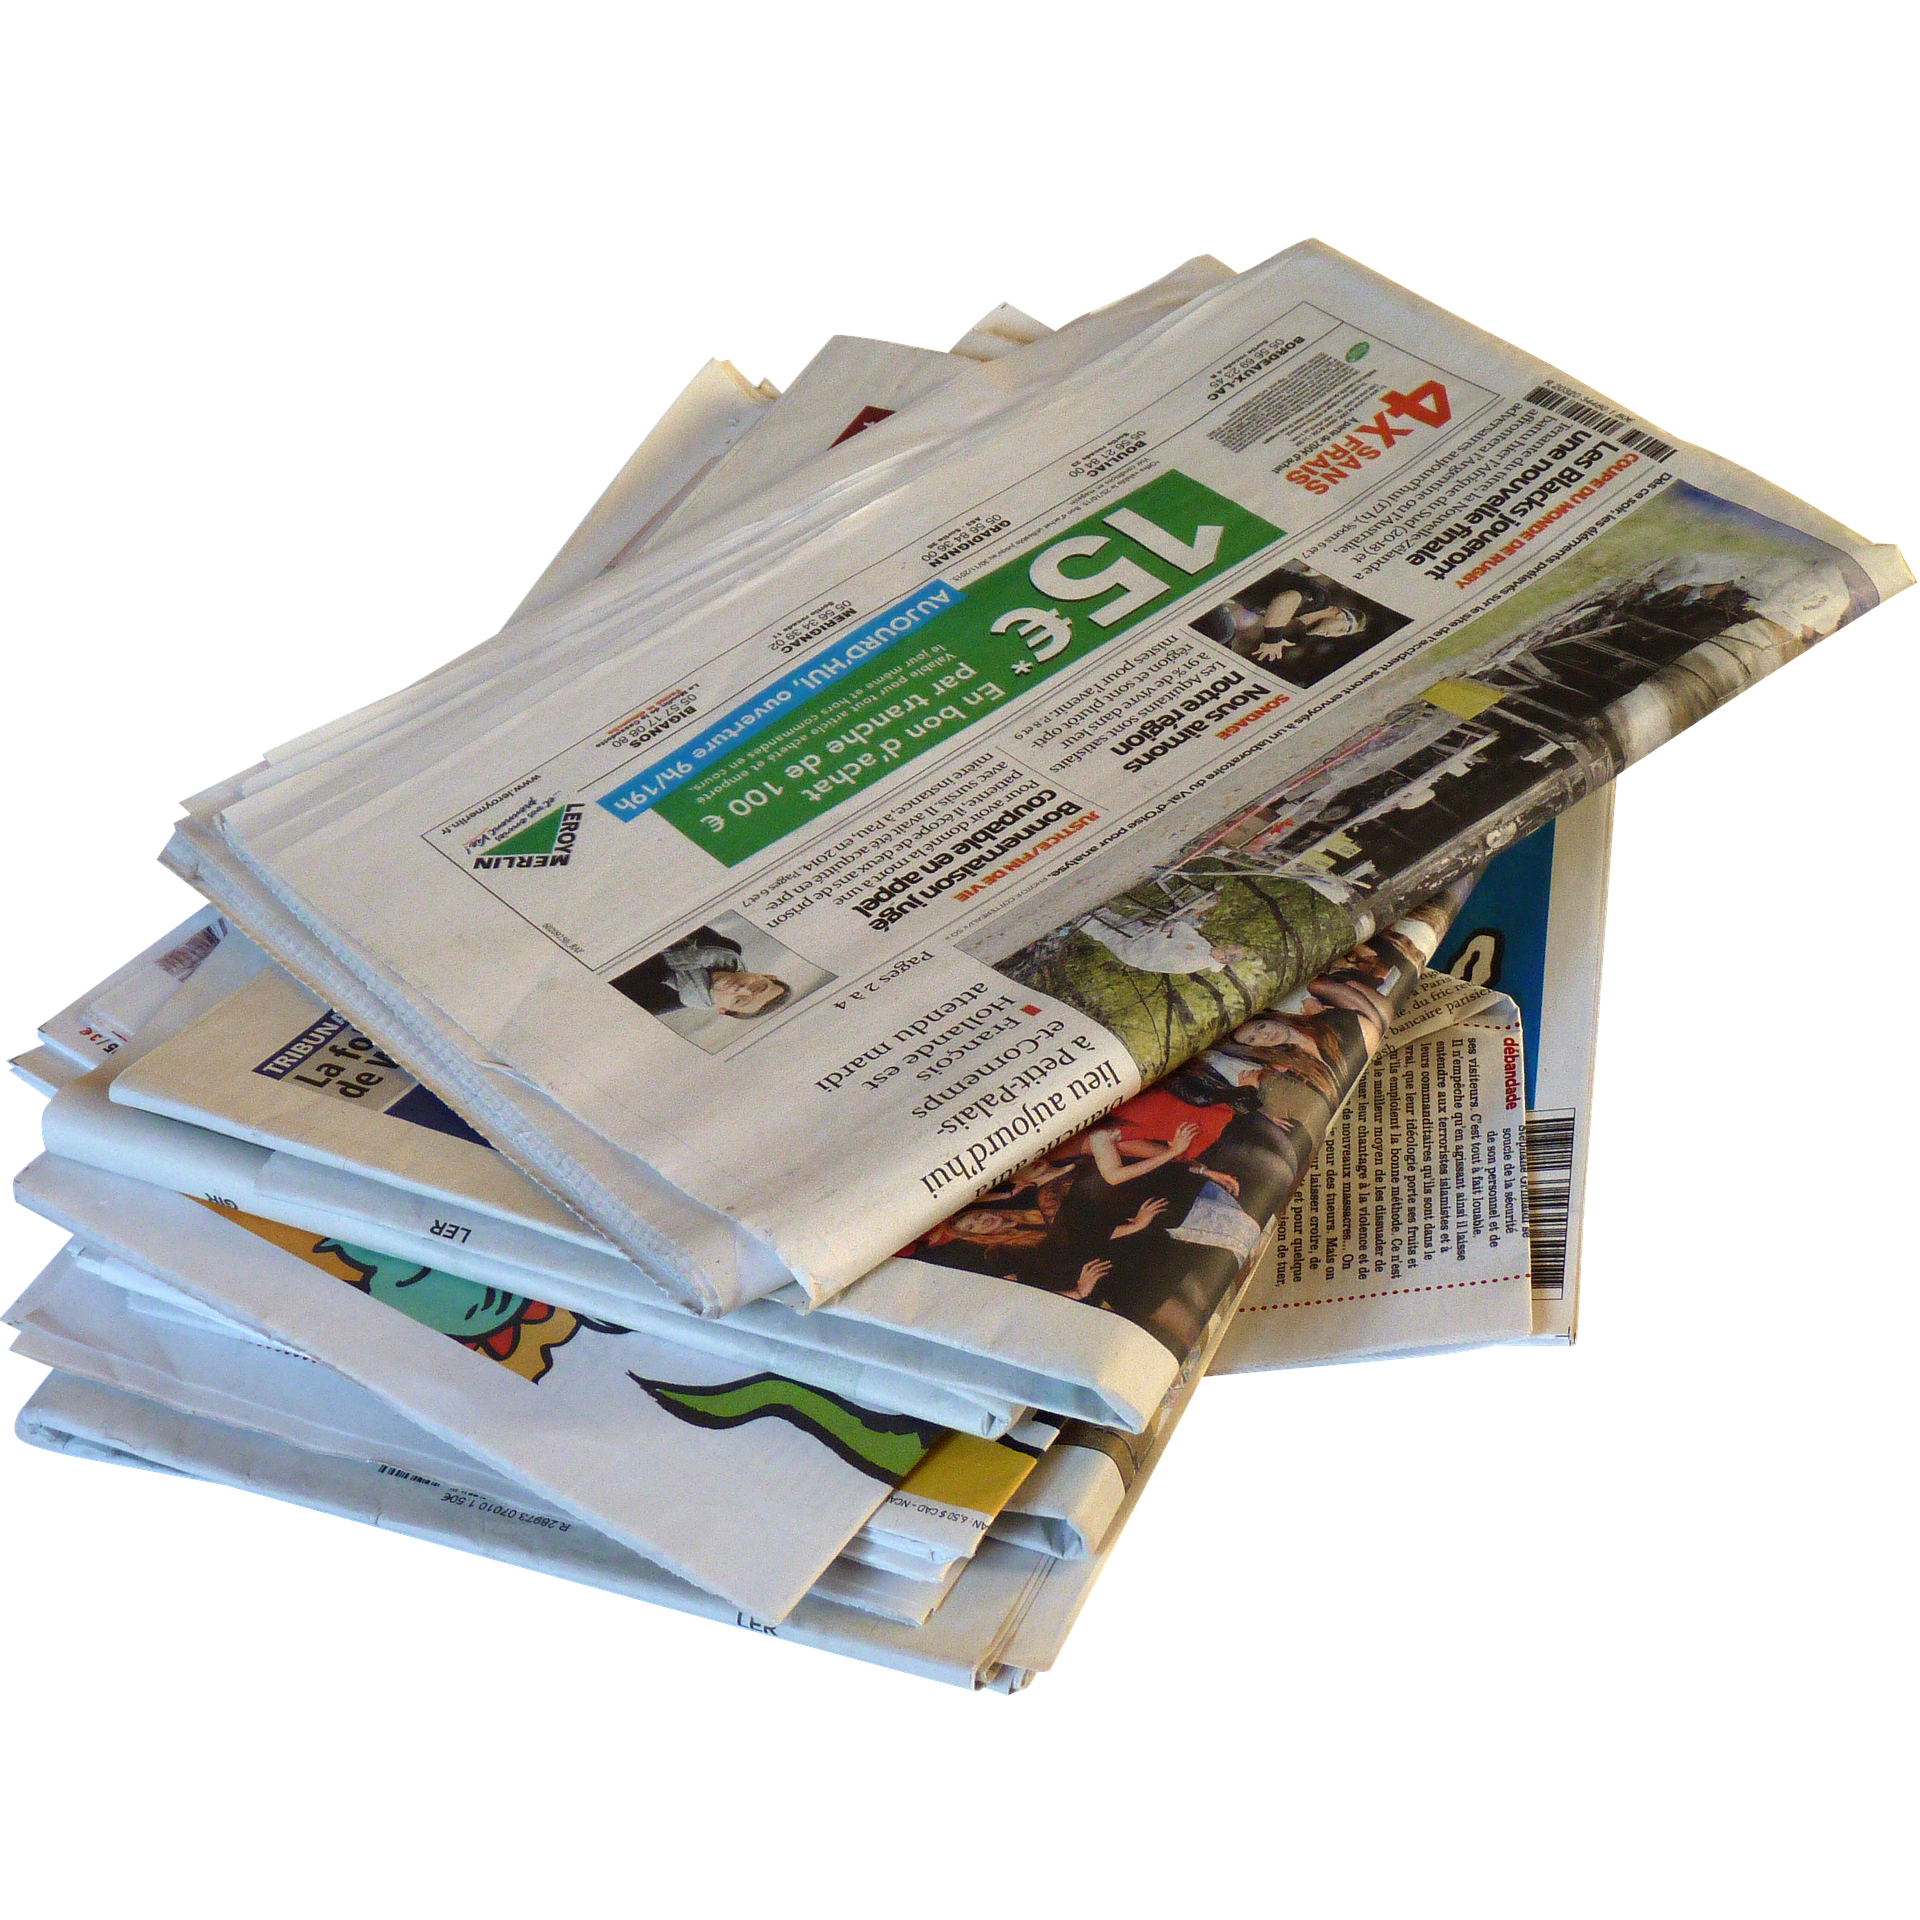
\includegraphics[width=\textwidth]{../SurvivalItemImages/newspaper}
        \end{minipage}\hfill
        \begin{minipage}{0.7\textwidth}
            \centering
            \Large Newspaper (one per person)
        \end{minipage}
    \end{figure}
    \vspace{-0.8em}
    \noindent\rule{\textwidth}{0.4pt}
            
    \begin{figure}[H]
        \centering
        \begin{minipage}{0.25\textwidth}
            \centering
            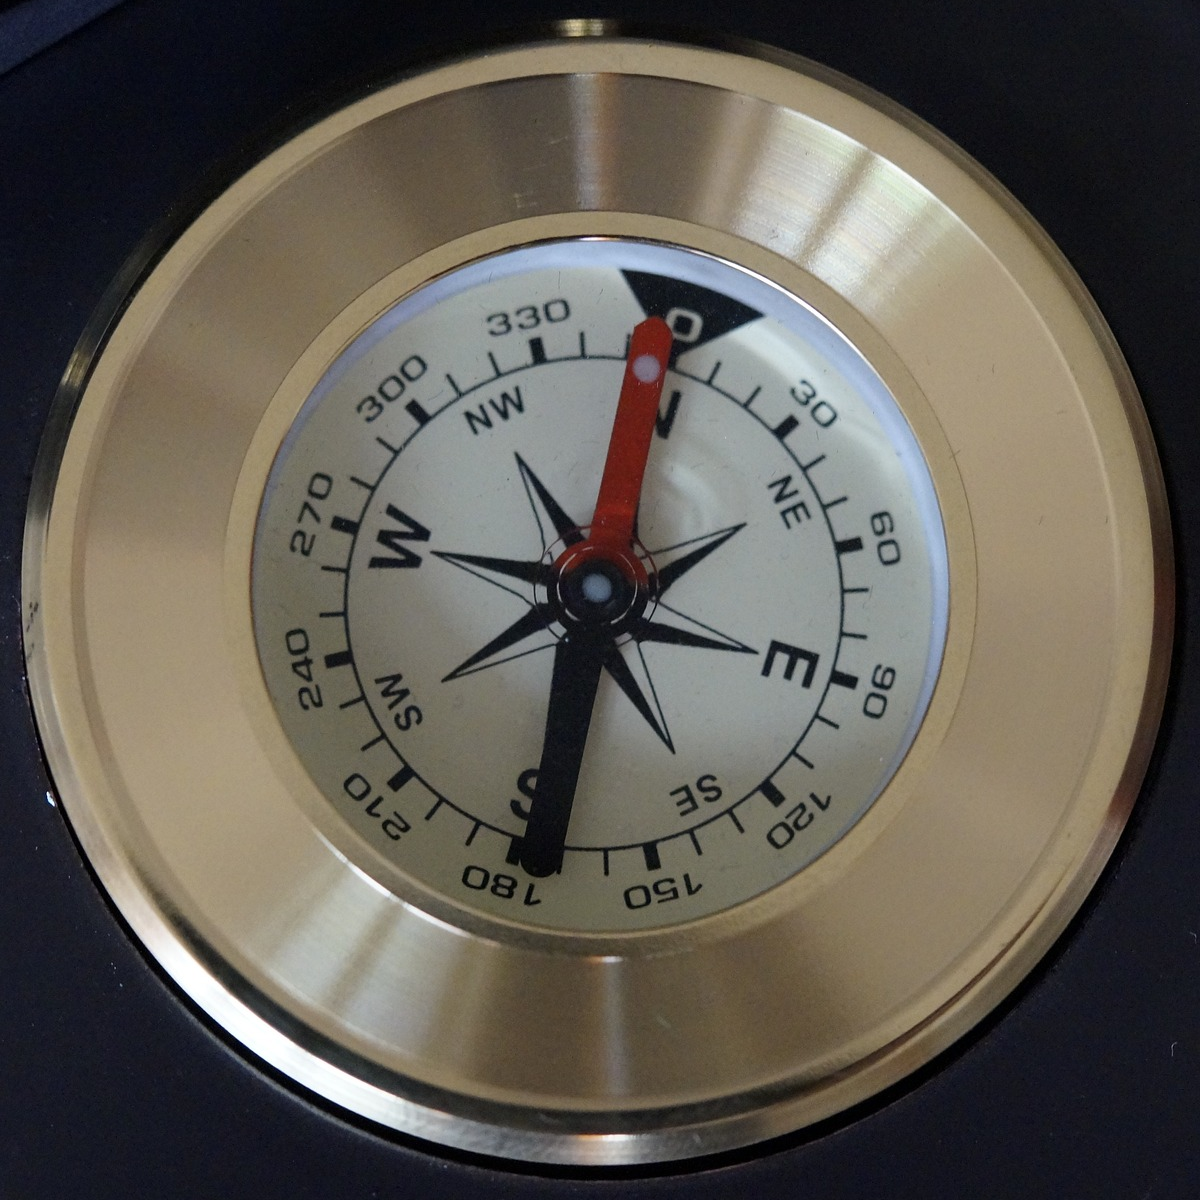
\includegraphics[width=\textwidth]{../SurvivalItemImages/compass}
        \end{minipage}\hfill
        \begin{minipage}{0.7\textwidth}
            \centering
            \Large Compass
        \end{minipage}
    \end{figure}
    \vspace{-0.8em}
    \noindent\rule{\textwidth}{0.4pt}
            
    \begin{figure}[H]
        \centering
        \begin{minipage}{0.25\textwidth}
            \centering
            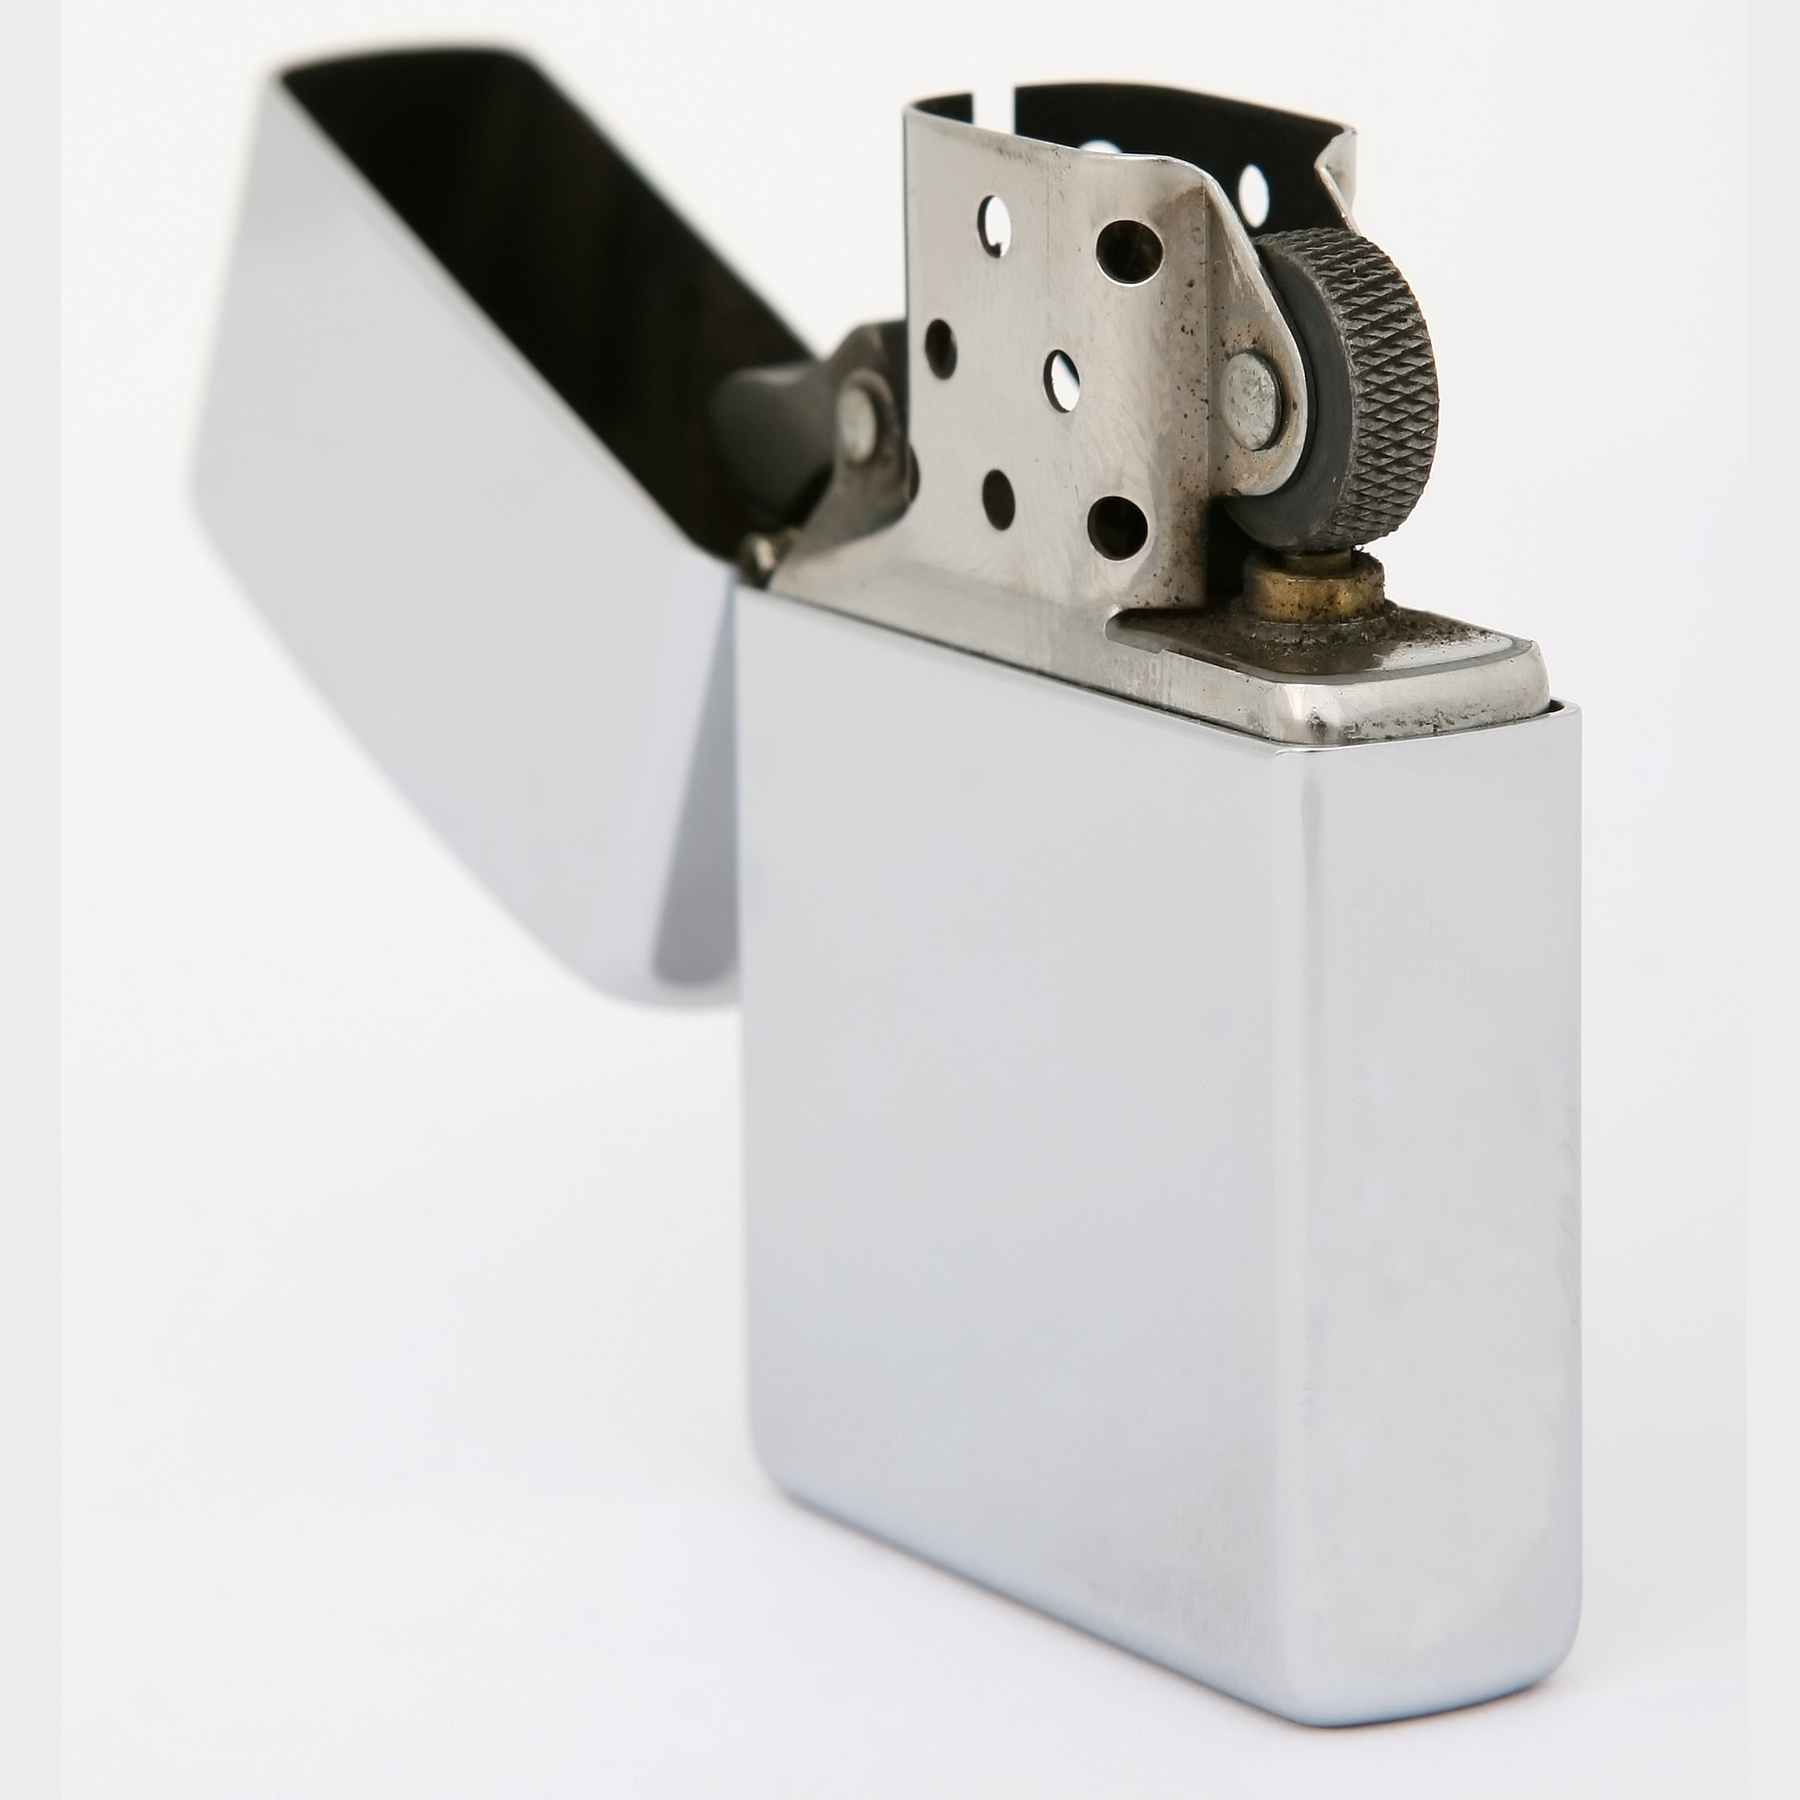
\includegraphics[width=\textwidth]{../SurvivalItemImages/lighter}
        \end{minipage}\hfill
        \begin{minipage}{0.7\textwidth}
            \centering
            \Large Cigarette lighter without the fluid
        \end{minipage}
    \end{figure}
    \vspace{-0.8em}
    \noindent\rule{\textwidth}{0.4pt}
            
    \begin{figure}[H]
        \centering
        \begin{minipage}{0.25\textwidth}
            \centering
            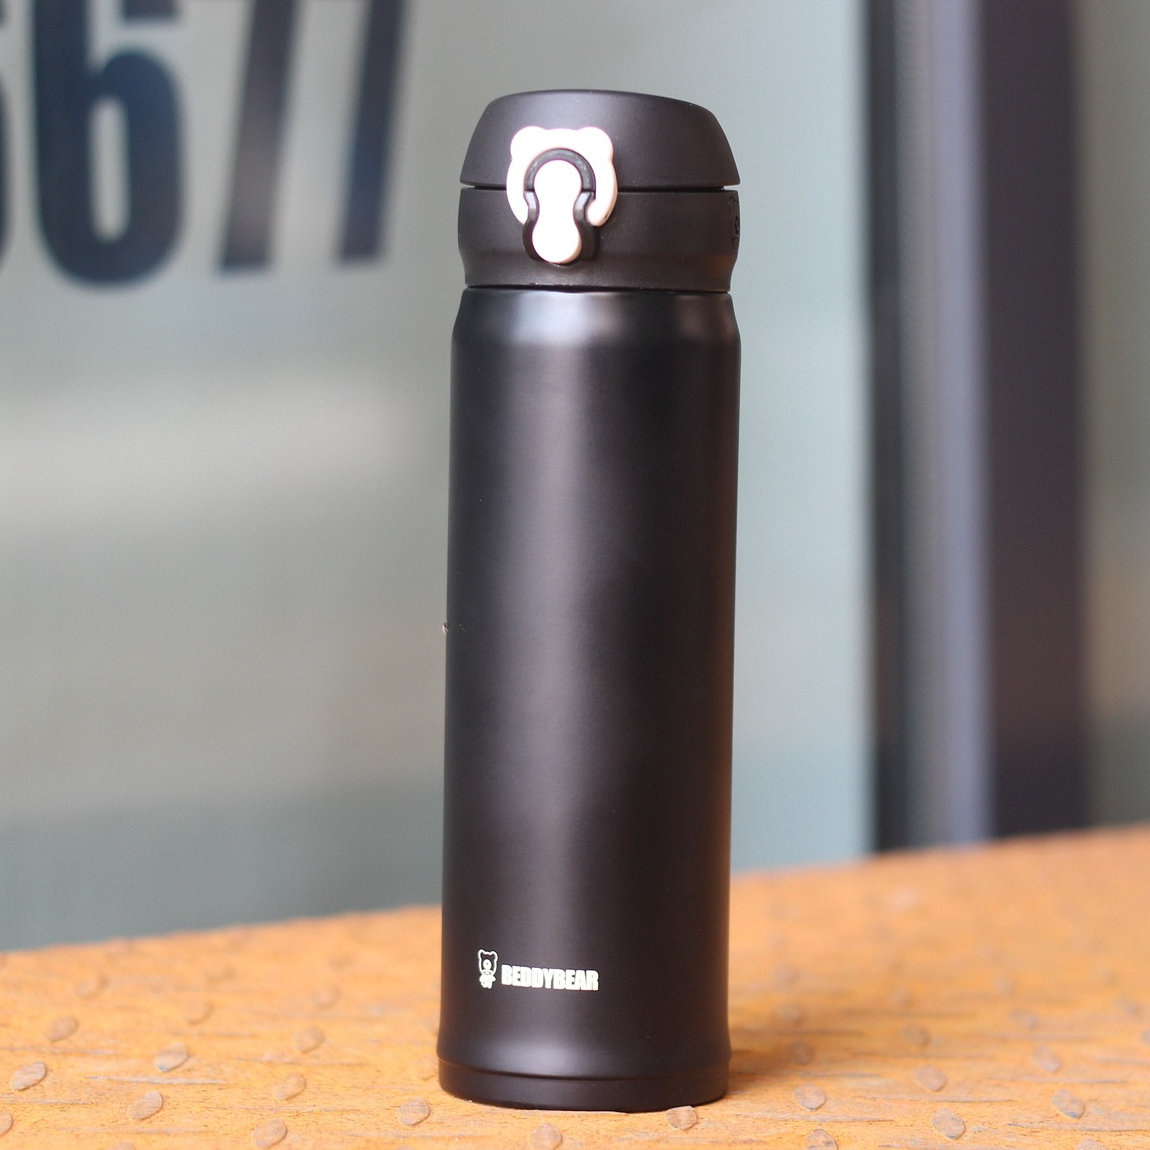
\includegraphics[width=\textwidth]{../SurvivalItemImages/thermos}
        \end{minipage}\hfill
        \begin{minipage}{0.7\textwidth}
            \centering
            \Large A thermos bottle
        \end{minipage}
    \end{figure}
    \vspace{-0.8em}
    \noindent\rule{\textwidth}{0.4pt}
            
    \clearpage
    \section*{Scenario: \textmd{Winter} \hfill Participant \textmd{2}}
    \Large You have just crash-landed in the North of Canada. The small plane in which you were travelling has been completely destroyed except for the frame. The pilot and co-pilot have been killed, but no one else is seriously injured.
You are in a wilderness area, snow-covered and made up of thick woods broken by many lakes and rivers. The pilot announced shortly before the crash that you were eighty miles northwest of a small town that is the nearest known habitation. It is mid-January. The last weather report indicated that the temperature would reach minus twenty-five degrees in the daytime and minus forty at night. You are dressed in winter clothing appropriate for city wear – suits, pantsuits, street shoes, and overcoats. While escaping from the plane, your group salvaged a few items.
\clearpage
        \end{document}
        